\documentclass{article}
\usepackage{amssymb}
\usepackage{amsmath}
\usepackage{centernot}
\usepackage{scalerel}
\usepackage{stackengine}
\usepackage{xcolor}
\usepackage{circuitikz}
\usepackage{graphicx}
\newcommand\showdiv[1]{\overline{\smash{\hstretch{.5}{)}\mkern-3.2mu\hstretch{.5}{)}}#1}}
\newcommand\ph[1]{\textcolor{white}{#1}}


\makeatletter
% we use \prefix@<level> only if it is defined
\renewcommand{\@seccntformat}[1]{%
  \ifcsname prefix@#1\endcsname
    \csname prefix@#1\endcsname
  \else
    \csname the#1\endcsname\quad
  \fi}
% define \prefix@section
\newcommand\prefix@section{}
\newcommand\prefix@subsection{}
\makeatother

\begin{document}

\title{Digital Logic Design: Homework 6}
\author{Joshua Dong}
\date{\today}
\maketitle

\section{9.1}
\subsection{a)}
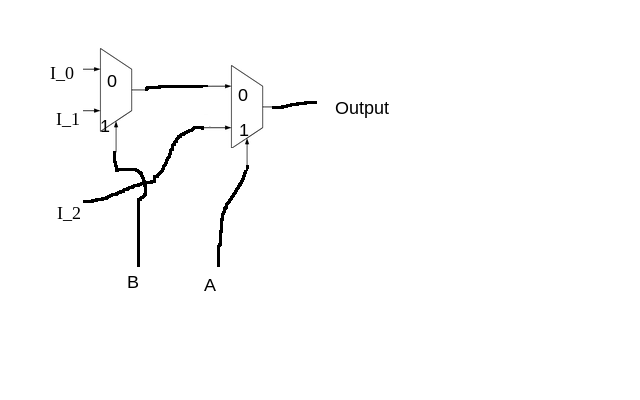
\includegraphics[scale=0.4]{23}
\subsection{b)}
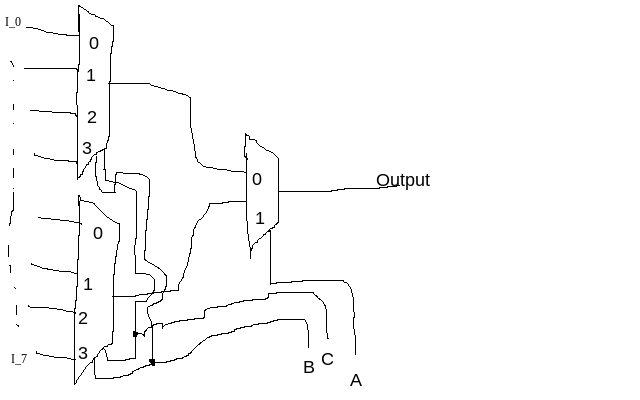
\includegraphics[scale=0.4]{4428}
\subsection{c)}
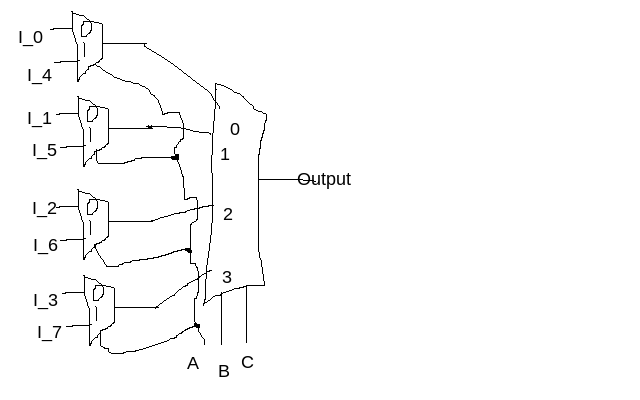
\includegraphics[scale=0.4]{222248}

\section{9.6}
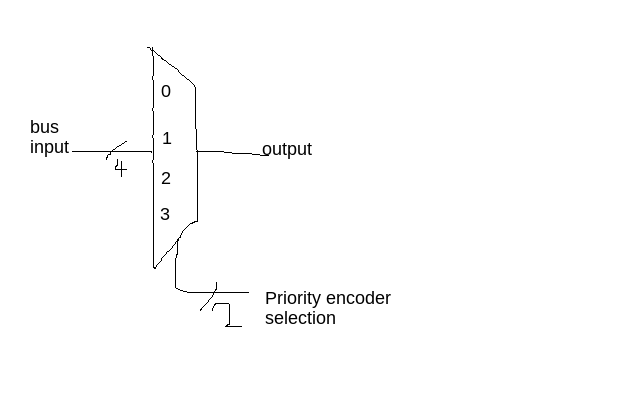
\includegraphics[scale=0.4]{bus}

\section{9.11}
\subsection{a)}
There are three products, requiring 3 AND gates. If $F$ is
inverted, $F' = (c'd' + bc' + a'c')' = (c' + d')(b + c')(a' + c') = ab'c'd + c$ then we only need 1 AND gate.
\subsection{b)}
If $F = a'b' + c'd'$, then we only need 2 AND gates. $F' = (a'b' + c'd') = bd + ab'd + bcd' + ab'cd'$, so we would need 4 AND gates for the inverted output.

\end{document}
